% 为了增强本研究的鲁棒性,我们在不同的显著性水平下检验了突变点的识别结果,发现在0.0005到0.05的置信度水平下,都只能识别出本研究发现的两个突变点(1978与2001)。
In order to enhance the robustness of this study, we tested the identification results of mutation points at different significance levels.
Our results that only two mutation points (1978 and 2001) could be identified at the confidence level of $0.0005$ to $0.05$ (Figure~\ref{fig:sensitivity}).
% 此外,我们讨论了在指标中没有体现的水库流量变化,在所有水库(图 x)中,我们分析了10个先后建成的枢纽水库,发现水库在 governance transforming regime 之后开始增强其调度的水平
In addition, we analyzed the changes of reservoir flow that are not reflected in the IWGI.\ Among all the reservoirs (Figure~\ref{fig:reservoirs}), we focused on $9$ major reservoirs built successively and find that the reservoirs began to enhance their variability after the governance transforming regime, suggesting a higher level of regulating (Figure~\ref{fig:conveyance}).

\begin{figure}[tb]
    \centering
    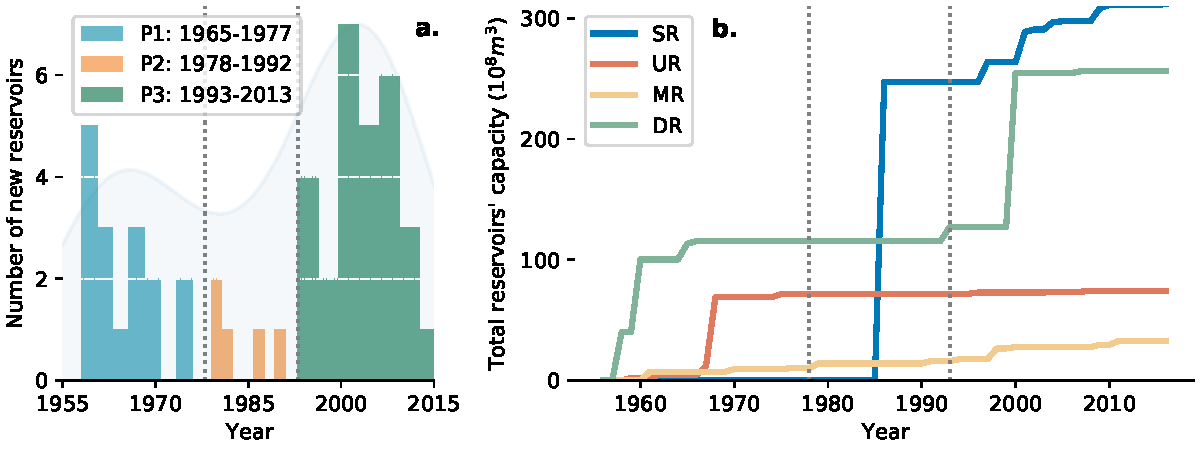
\includegraphics[width=0.6\linewidth]{sup/reservoirs.pdf}
    \caption{
          Numbers of new reservoirs in each year.
    }\label{fig:reservoirs}
\end{figure}

\begin{figure}
    \centering
    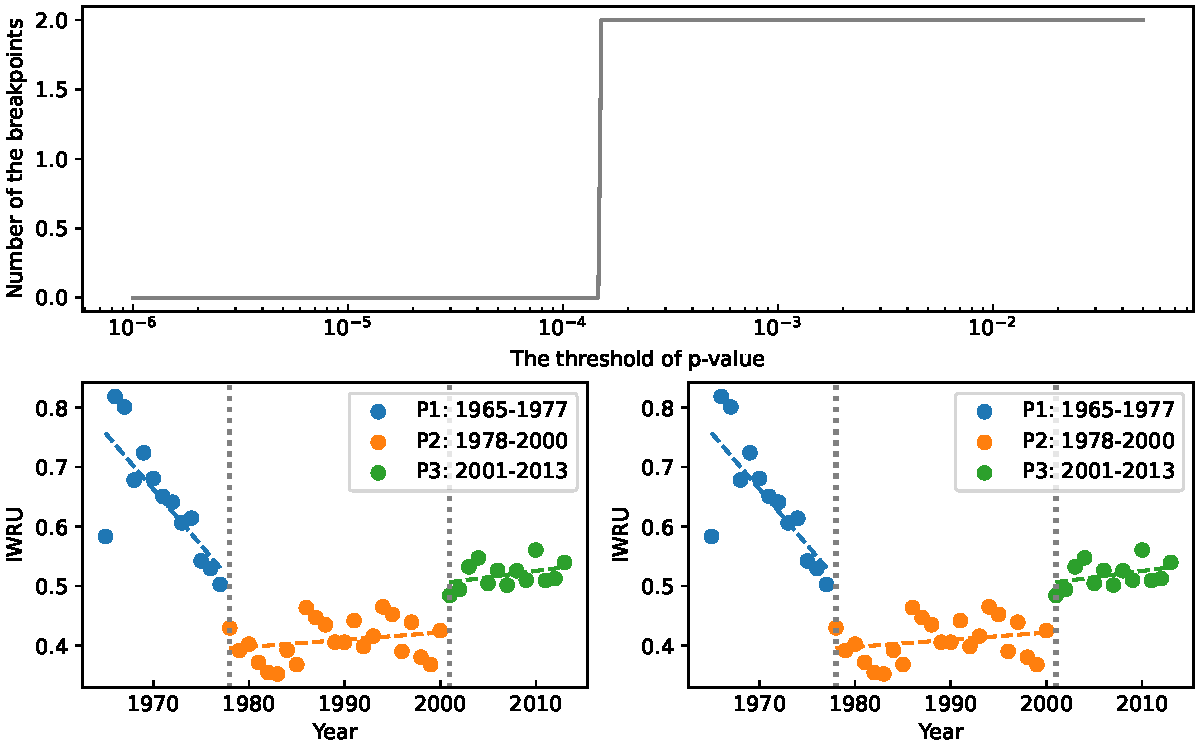
\includegraphics[width=\linewidth]{sup/sensitivity.pdf}
    \caption{
          Sensitivity analysis of the threshold of p-values.
          \textbf{A.} number of breakpoints in different p-values, the scheme with two-breakpoints are the dominant situation.
          \textbf{B.} Threshold of p-values \(\alpha=0.0005\).
          \textbf{C.} Threshold of p-values \(\alpha=0.05\).
    }\label{fig:sensitivity}
\end{figure}


\begin{figure}[htb]
    \centering
    \includegraphics[width=0.8\textwidth]{sup/conveyance.png}
    \caption{Monthly conveyance flow differences of the reservoirs mainly for managing and regulating the whole basin and their variability}\label{fig:conveyance}
\end{figure}
